\subsubsection{Descripción}

En esta sección trataremos de encontrar cuáles son los parámetros que optimizan los resultados de KNN al preprocesar la información usando PCA y PLS-DA. Para esto tendremos en cuenta los tiempos de ejecución de los algoritmos para encontrar la mejor relación entre calidad y costo temporal.

\subsubsection{PCA}

\subsubsection*{Costo temporal}

Al igual que en el experimento anterior, la variación de k no altera significativamente el costo temporal de KNN. Por lo tanto para analizarlo, nos preocuparemos de calcular únicamente el rango ideal de valores para el parámetro alpha. Los siguientes gráficos muestran exactamente eso.

\begin{figure}[h!]
  \begin{center}
	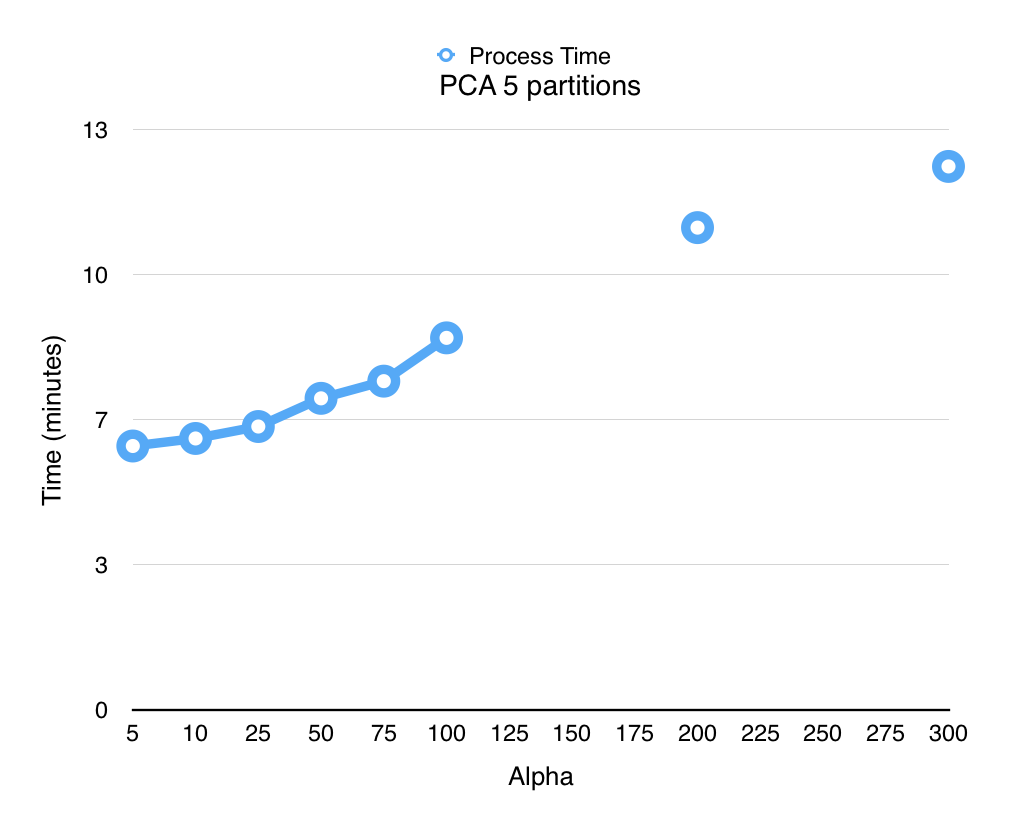
\includegraphics[scale=0.7]{exp2/PCA-Process-Time.png}
	\caption{PCA data set training}
%	\label{accum_var_PCA}
  \end{center}
\end{figure}

En este gráfico podemos ver el tiempo que lleva el entrenamiento de PCA para reducir la dimensión de los vectores. Para algunos valores intermedios no fue calculado este valor debido al tiempo de cómputo que se requería, pero de todos modos podemos percibir una complejidad aproximadamente lineal, al menos en el rango que nos compete.

\newpage
\begin{figure}[h!]
  \begin{center}
	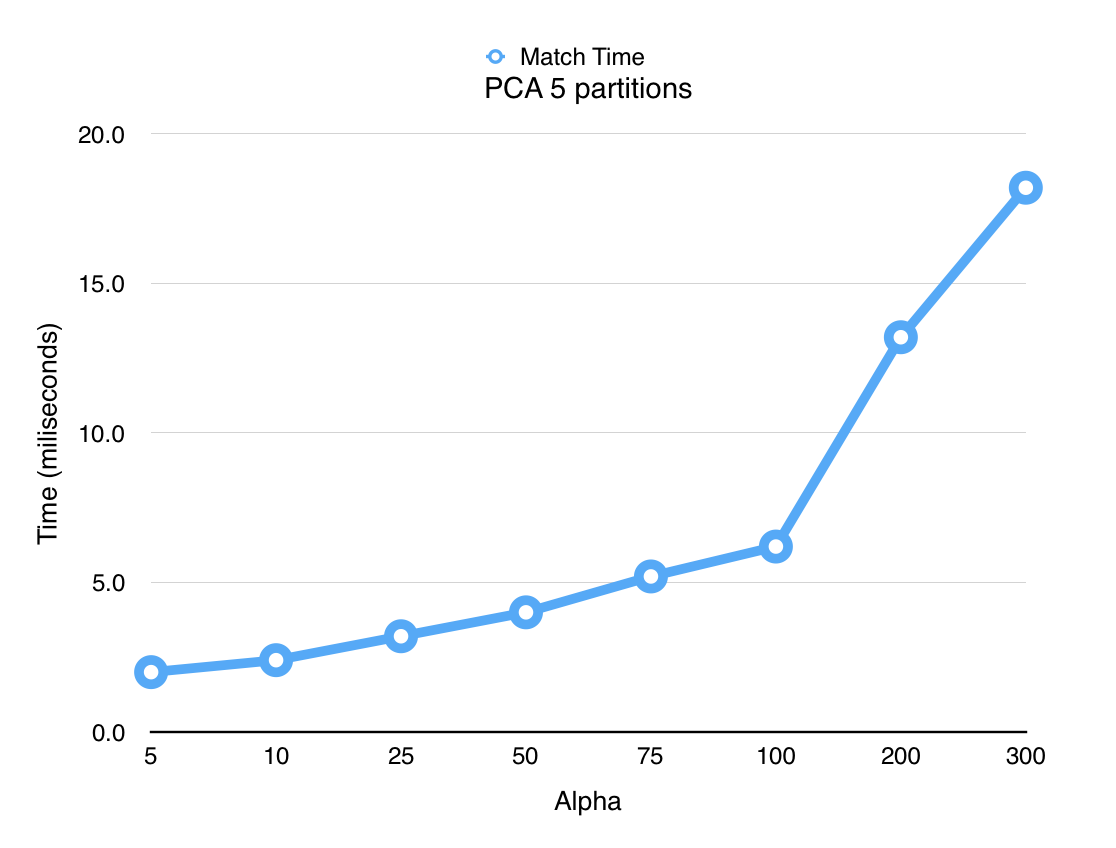
\includegraphics[scale=0.7]{exp2/PCA-Match-Time.png}
	\caption{KNN Image Process Duration After PCA}
%	\label{accum_var_PCA}
  \end{center}
\end{figure}

En este otro gráfico se aprecia el tiempo en milisegundos que tarda una nueva imagen en ser clasificada usando KNN + PCA, una vez entrenado el data set. En este caso también podemos notar la linealidad de la función.

Por lo tanto podemos concluir que en los rangos adecuados, la complejidad temporal tanto del entrenamiento como de la clasificación es lineal respecto a alpha. Por lo tanto emprendemos el análisis de la calidad de los resultados teniendo este factor en cuenta.

\subsubsection*{Calidad del algoritmo}

\begin{table}[h!]
\begin{center}
\begin{tabular}{c c}
	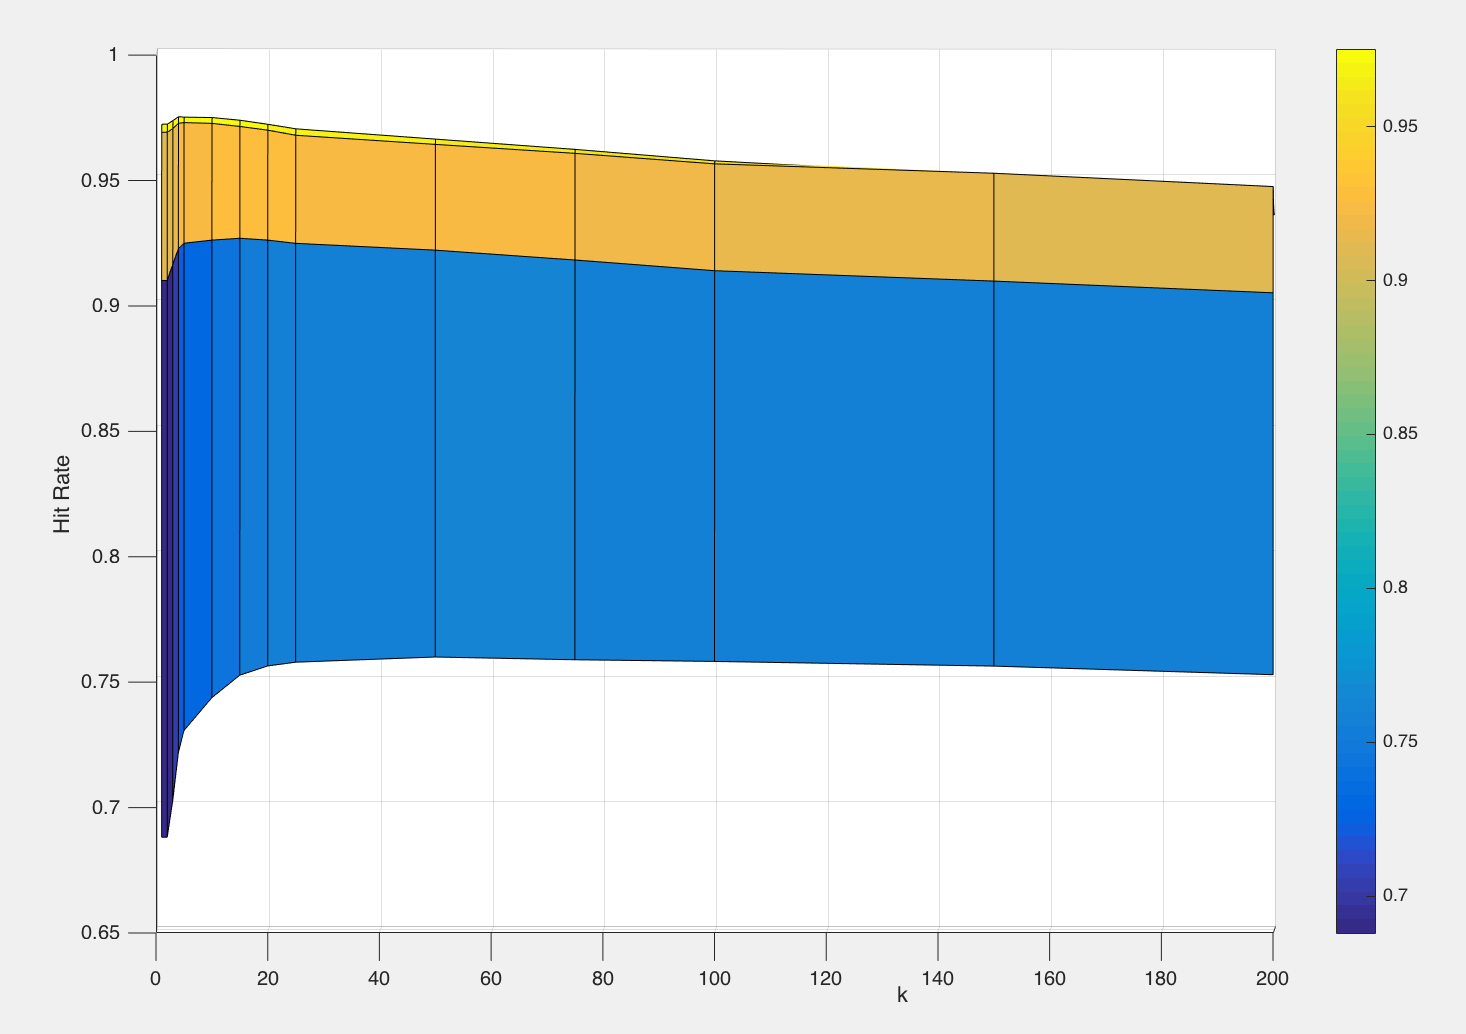
\includegraphics[scale=0.3]{exp2/PCA-HitRate-1.png} &
	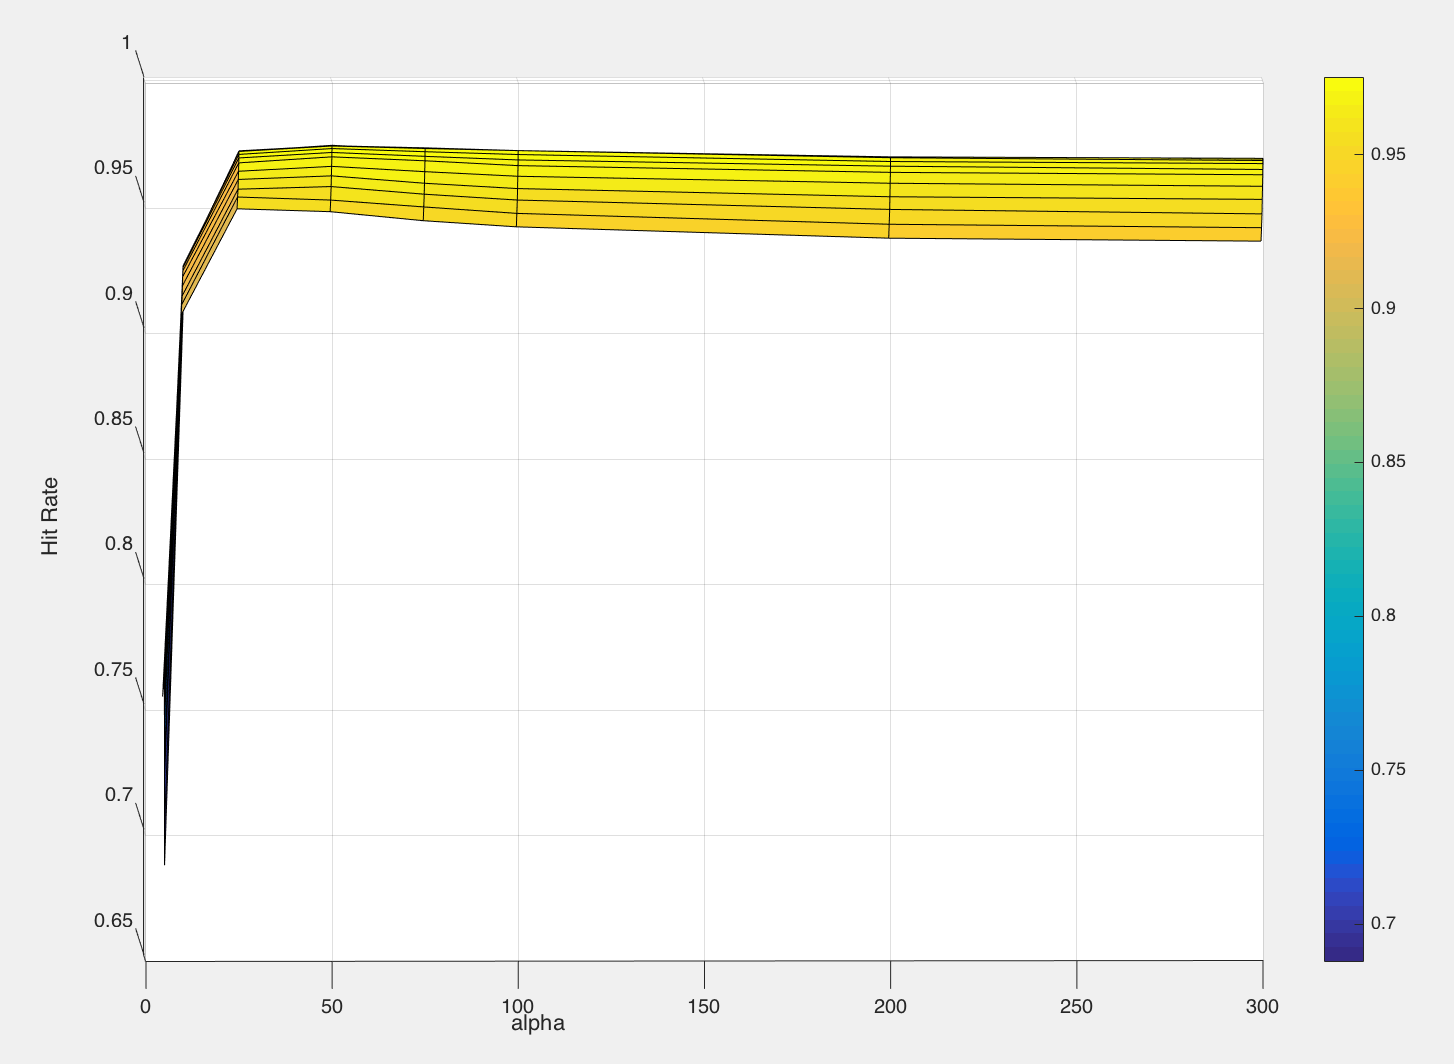
\includegraphics[scale=0.3]{exp2/PCA-HitRate-2.png}\\
\end{tabular}
\end{center}
\caption{Hit Rate para valores de $alpha$ y $k$}
\end{table}

\begin{figure}[h!]
  \begin{center}
	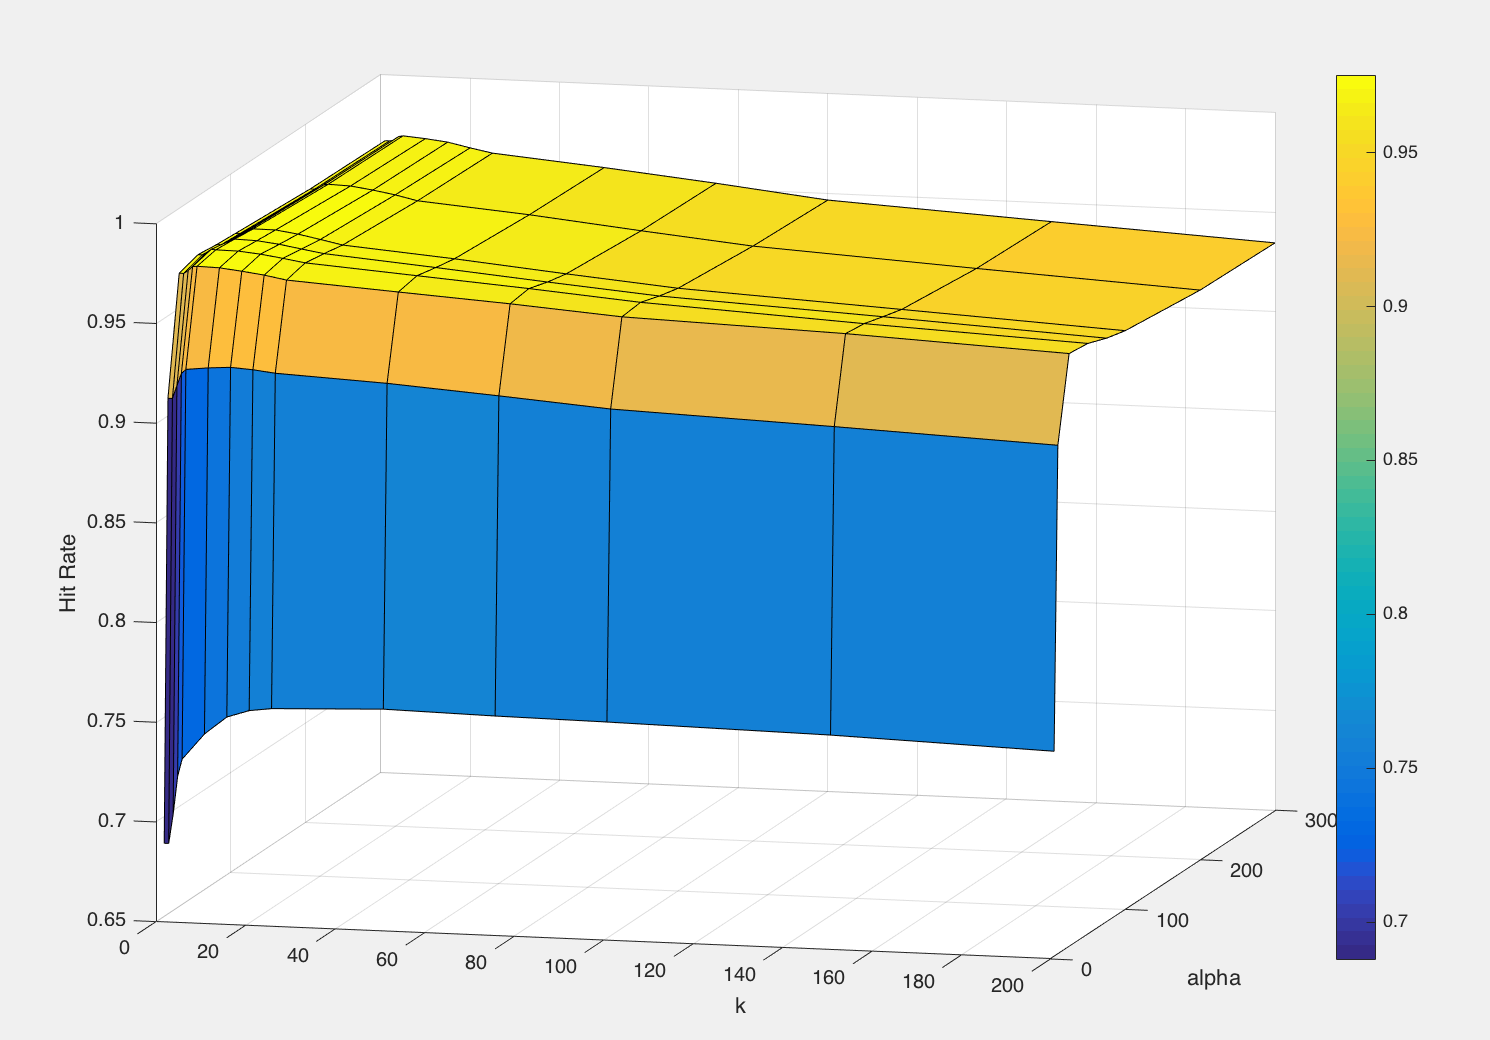
\includegraphics[scale=0.5]{exp2/PCA-HitRate-3.png}
	\caption{PCA data set training}
%	\label{accum_var_PCA}
  \end{center}
\end{figure}

En estas figuras graficamos los valores del hit rate para valores de $alpha$ entre 5 y 300, y de $k$ entre 1 y 200. Las primeras 2 figuras nos muestran los perfiles. 

En la primera se puede observar la curva para los valores de $k$. Estos tienen un pico en $k = 4$ y luego comienza a descender. Esto al igual que en KNN puro se debe probablemente a que agregar muchos vecinos empieza a generar ruido en la clasificación de la imagen. Vemos que pocos vecinos tampoco generan el resultado óptimo.

Por otro lado en la segunda imagen vemos cómo fluctúa el hit rate respecto a alpha. En este caso es interesante ver que menos de 10 autovectores dan un resultado bastante pobre y que encontramos un máximo en $alpha = 50$. A partir de ahí el hit rate comienza a descender. Esto es contraintuitivo ya que en teoría al aumentar el alpha estamos dando más información. Es probable que la información que comienzan a dar los nuevos autovectores ensucien más de lo que ayudan.

En el último gráfico tenemos una vista más general de ambos parámetros. Aquí se puede ver que tenemos nuestro máximo en $alpha = 50$ y $k = 4$. Lo interesante es que no hay que comprometer demasiado el tiempo de cómputo con ese alpha.

\subsubsection{PLS-DA}

\subsubsection*{Costo temporal}

Al igual que para PCA, nos centramos en analizar valores de gamma únicamente para determinar un rango adecuado de valores a considerar. Las siguientes imágenes muestran los resultados obtenidos.

\begin{figure}[h!]
  \begin{center}
	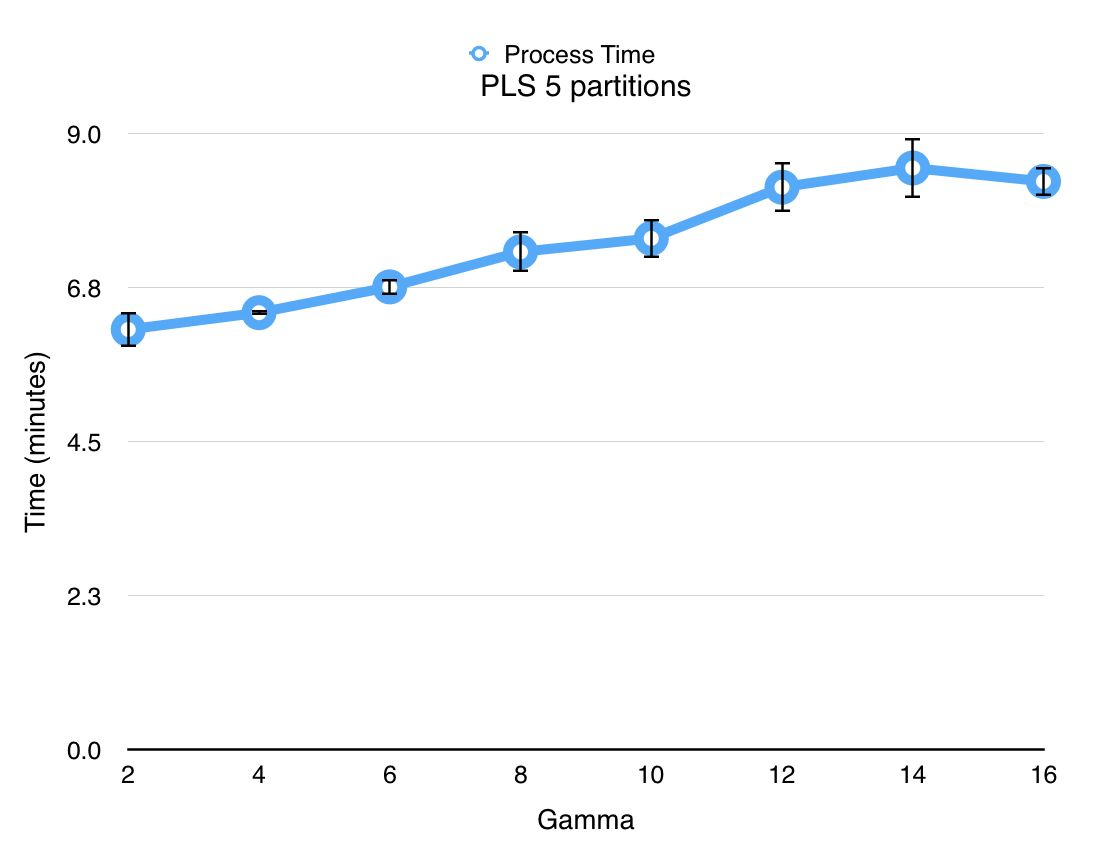
\includegraphics[scale=0.7]{exp2/PLS-Process-Time.png}
	\caption{PLS-DA data set training}
%	\label{accum_var_PCA}
  \end{center}
\end{figure}

En esta imagen se puede apreciar también cierta linealidad en el costo temporal del entrenamiento de PLS. Vemos incluso que el desvío estándar es bastante pequeño entre las particiones así que el gráfico es bastante representativo.

\begin{figure}[h!]
  \begin{center}
	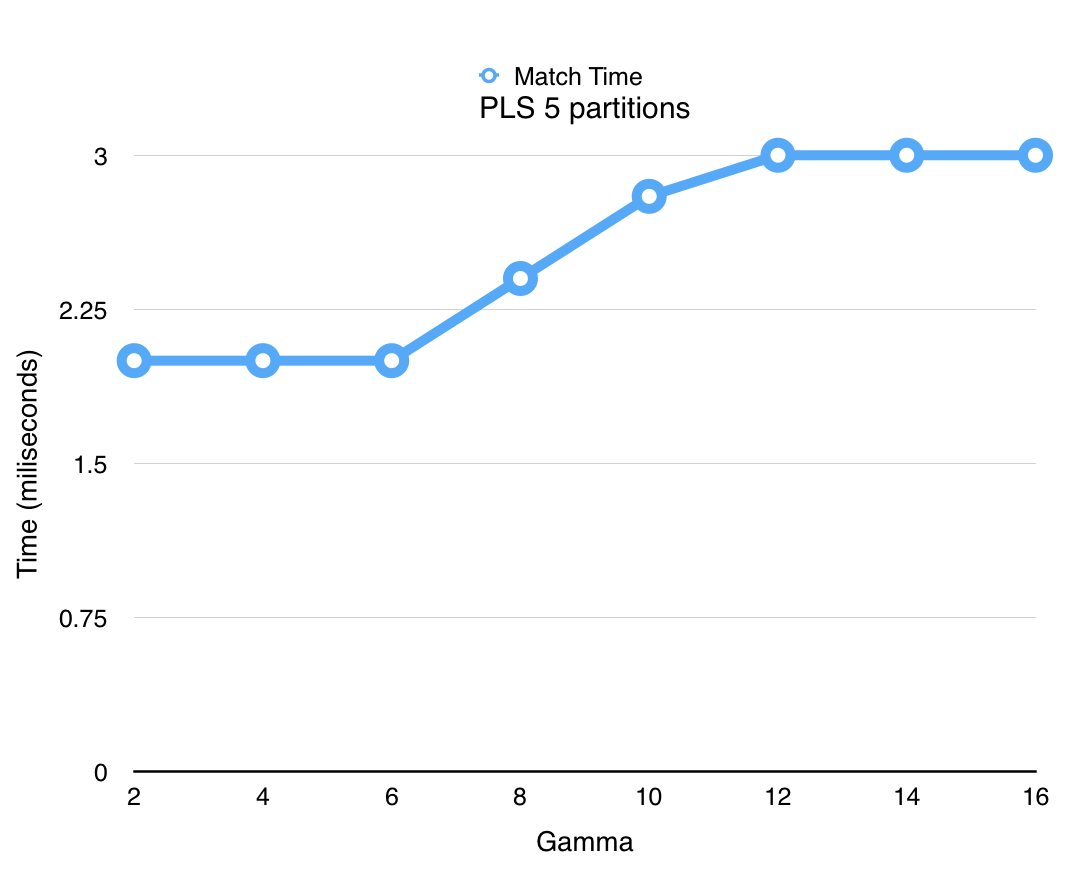
\includegraphics[scale=0.7]{exp2/PLS-Match-Time.png}
	\caption{PLS-DA data set training}
%	\label{accum_var_PCA}
  \end{center}
\end{figure}

Por otro lado en esta imagen se puede ver que el tiempo de clasificación de una nueva imagen tiene un comportamiento bastante estacionario. Se ve que entre gamma 6 y 12 el costo temporal aumenta rápidamente.












